%% LyX 2.2.2 created this file.  For more info, see http://www.lyx.org/.
%% Do not edit unless you really know what you are doing.
\documentclass[11pt,italian,handout]{beamer}
\usepackage{lmodern}
\renewcommand{\sfdefault}{lmss}
\renewcommand{\ttdefault}{lmtt}
\usepackage[T1]{fontenc}
\usepackage[utf8]{inputenc}
\setcounter{secnumdepth}{3}
\setcounter{tocdepth}{3}
\usepackage{textcomp}
\usepackage{amsmath}
\usepackage{amssymb}
\usepackage{graphicx}

\makeatletter

%%%%%%%%%%%%%%%%%%%%%%%%%%%%%% LyX specific LaTeX commands.
\pdfpageheight\paperheight
\pdfpagewidth\paperwidth

%% A simple dot to overcome graphicx limitations
\newcommand{\lyxdot}{.}


%%%%%%%%%%%%%%%%%%%%%%%%%%%%%% Textclass specific LaTeX commands.
 % this default might be overridden by plain title style
 \newcommand\makebeamertitle{\frame{\maketitle}}%
 % (ERT) argument for the TOC
 \AtBeginDocument{%
   \let\origtableofcontents=\tableofcontents
   \def\tableofcontents{\@ifnextchar[{\origtableofcontents}{\gobbletableofcontents}}
   \def\gobbletableofcontents#1{\origtableofcontents}
 }
 % plain title style, override default
 \renewcommand\makebeamertitle{\frame[plain]{\maketitle}}%

%%%%%%%%%%%%%%%%%%%%%%%%%%%%%% User specified LaTeX commands.
\usepackage{microtype}
\usepackage{pgf,tikz}
\usepackage{pstricks}
\usepackage{pstricks-add}
\usetikzlibrary{arrows}
\usetheme{Frankfurt}
\definecolor{blue1}{RGB}{51,51,179}
\definecolor{blue2}{RGB}{0,0,204}
\definecolor{blue3}{RGB}{0,0,153}
\setbeamercolor{author in head/foot}{fg=white, bg=blue3}
\setbeamercolor{title in head/foot}{fg=white, bg=blue2}
\setbeamercolor{date in head/foot}{fg=white, bg=blue1}
\useoutertheme{split}
\setbeamertemplate{navigation symbols}{}
\setbeamertemplate{footline}
{
  \leavevmode%
  \hbox{%
  \begin{beamercolorbox}[wd=.333333\paperwidth,ht=2.25ex,dp=1ex,center]{author in head/foot}%
    \usebeamerfont{author in head/foot}\insertshortauthor~~\beamer@ifempty{\insertshortinstitute}{}{(\insertshortinstitute)}
  \end{beamercolorbox}%
  \begin{beamercolorbox}[wd=.333333\paperwidth,ht=2.25ex,dp=1ex,center]{title in head/foot}%
    \usebeamerfont{title in head/foot}\insertshorttitle
  \end{beamercolorbox}%
  \begin{beamercolorbox}[wd=.333333\paperwidth,ht=2.25ex,dp=1ex,right]{date in head/foot}%
    \usebeamerfont{date in head/foot}\insertshortdate{}\hspace*{2em}
    \insertframenumber{} / \inserttotalframenumber\hspace*{2ex} 
  \end{beamercolorbox}}%
  \vskip0pt%
}
\usepackage[absolute,overlay]{textpos}
\setlength{\TPHorizModule}{1mm}
  \setlength{\TPVertModule}{1mm}
\newcommand\Fontvi{\fontsize{8}{12}\selectfont}

\makeatother

\usepackage{babel}
\begin{document}

\title{Dinamica epidemica su reti adattative}

\subtitle{Thilo Gross, Carlos Dommar D'Lima, and Bernd Blasius}

\author{Gabriele Vanoni}

\institute{Politecnico di Milano}

\date{6 Aprile 2017}
\makebeamertitle

\section{Introduzione}
\begin{frame}[plain]
\begin{center}
\textbf{\LARGE{}Introduzione}
\par\end{center}{\LARGE \par}

\end{frame}
\begin{frame}{I punti di partenza}

\begin{textblock}{60}(10,15)
\begin{block}{Modelli generativi di reti complesse}
\begin{itemize}
\item Reti \textbf{small world} attraverso ``rewiring selettivo'' {[}Watts
e Strogatz, \textit{Nature}, 1998{]}
\item Reti \textbf{scale-free} attraverso ``attaccamento preferenziale''
{[}Barabasi e Albert, \textit{Science}, 1999{]}
\end{itemize}
\end{block}
%
\begin{block}{Modello SIS su rete {[}Pastor-Satorras e Vespignani, \textit{Phys.
Rev. Lett.}, 2001{]}}

La \textbf{topologia} della rete influenza la dinamica di diffusione
dell'epidemia.
\end{block}
\end{textblock}

\begin{textblock}{30}(75,12)

\includegraphics[scale=0.3]{393440aa\lyxdot eps\lyxdot 2}

{\tiny{}Watts e Strogatz, }\textit{\tiny{}Nature}{\tiny{}, 1998}{\tiny \par}

\smallskip{}

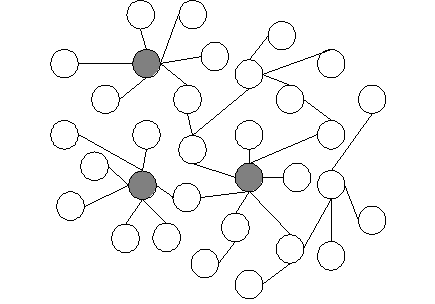
\includegraphics[scale=0.3]{Scale-free_network_sample}

{\tiny{}Castiglio,}\textit{\tiny{} PhD Thesis}{\tiny{}, 2004}{\tiny \par}

\smallskip{}

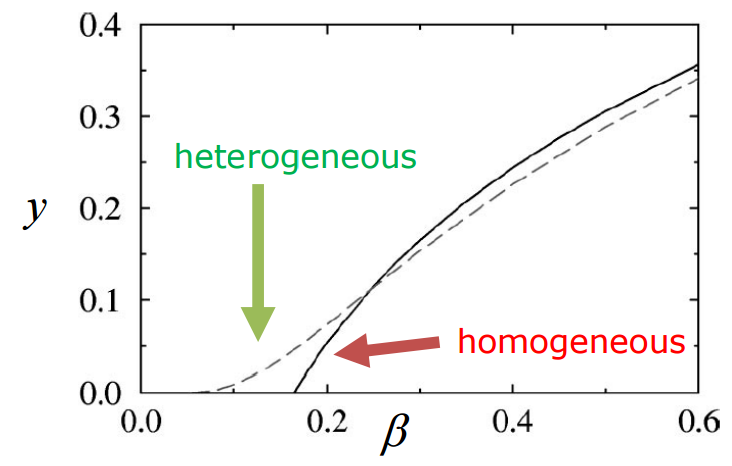
\includegraphics[scale=0.15]{soglia2}

{\tiny{}Piccardi, }\textit{\tiny{}Lett. Mat. Int}{\tiny{}., 2013}{\tiny \par}

\end{textblock}
\end{frame}
%
\begin{frame}{L'idea}
\begin{block}{Reti adattative}

Chiamiamo una rete \textbf{adattativa} (o coevolutiva) se è in grado
di modificare la propria topologia dinamicamente in risposta allo
stato dinamico dei nodi.\pause
\end{block}
\bigskip{}

\begin{center}
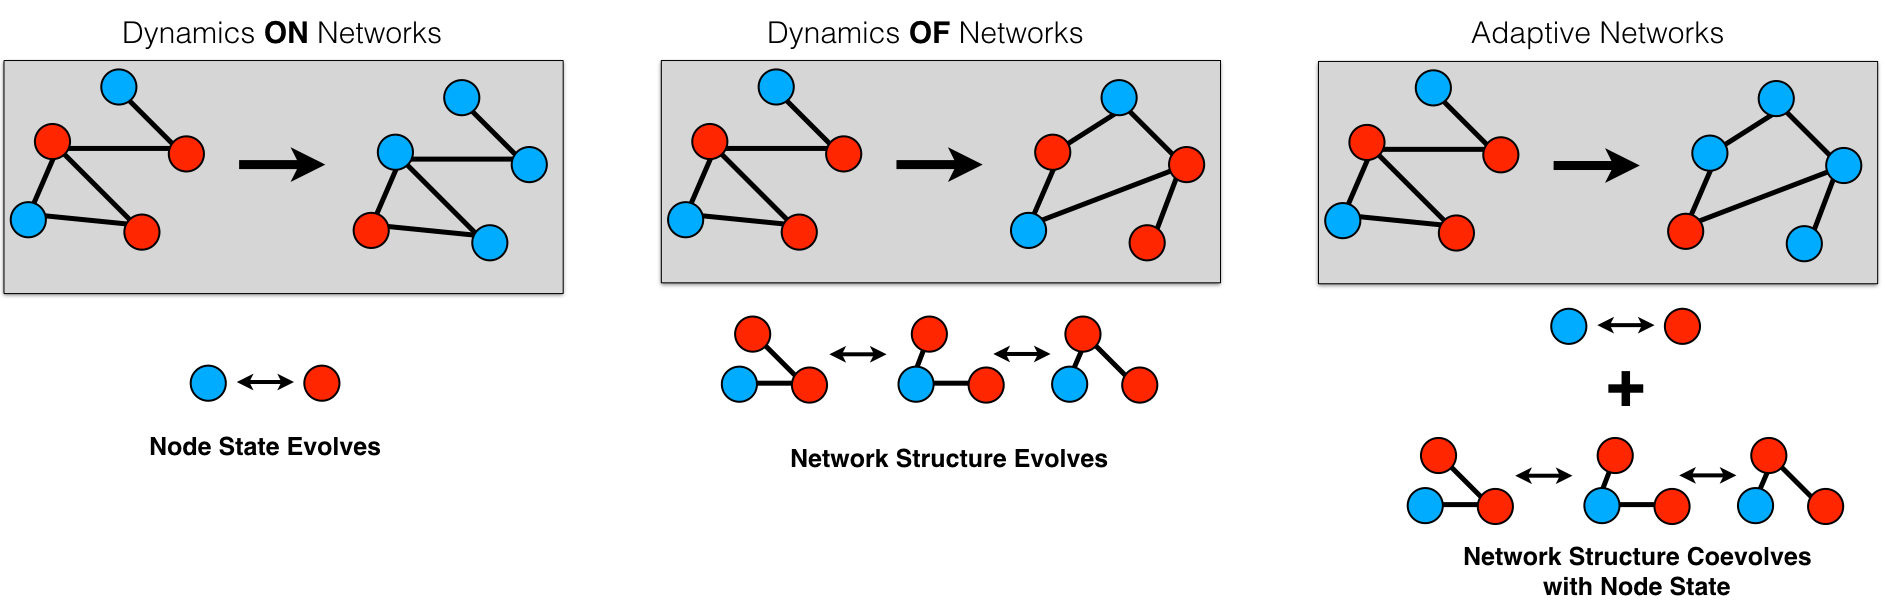
\includegraphics[scale=0.16]{fdistnet1}
\par\end{center}

\vspace{-1cm}

\begin{center}
{\tiny{}Nishant Malik and Feng Shi, }\textit{\tiny{}DSWeb}{\tiny{},
2017}
\par\end{center}{\tiny \par}
\end{frame}

\section{Modello}
\begin{frame}[plain]
\begin{center}
\textbf{\LARGE{}Modello}
\par\end{center}{\LARGE \par}

\end{frame}
\begin{frame}{Definizione del modello}
\begin{block}{Definizione}
\begin{itemize}
\item Consideriamo una rete non diretta, non pesata con $N$ nodi e $K$
link.
\item Ogni nodo può essere suscettibile (S) o infetto (I).
\item Ad ogni intervallo di tempo $\Delta t$, per ogni link SI, il nodo
suscettibile diventa infetto con probabilità $p$ costante.
\item Ad ogni intervallo di tempo $\Delta t$, gli infetti si riprendono
dalla malattia ritornando suscettibili con probabilità $r$ costante.
\item Ad ogni intervallo di tempo $\Delta t$, i suscettibili redirigono
con probabilità $w$ ogni link SI verso un suscettibile scelto a caso
(auto-anelli e doppie connessioni non sono permessi).
\end{itemize}
\end{block}
\end{frame}
%
\begin{frame}{Effetti del rewiring sulla stabilità dell'epidemia}

Chiamiamo:
\begin{block}{}

\begin{itemize}
\item $p^{*}$ la\textbf{ probabilità soglia di infezione} necessaria a
mantenere stabile l'epidemia.\pause
\item $R_{0}$ il \textbf{basic reproductive number} ovvero il numero di
nodi infettati da un singolo nodo infetto immerso in una rete di suscettibili.\pause
\end{itemize}
\end{block}
In una rete \textbf{casuale senza rewiring} $R_{0}=\frac{p\left\langle k\right\rangle }{r}$.\pause

Diciamo che l'epidemia è stabile se $R_{0}=1$, da cui $p^{*}=\frac{r}{\left\langle k\right\rangle }$.\pause

\bigskip{}

Considerando che il \textbf{rewiring} fa perdere in media a un nodo
infetto una frazione costante $w$ di link il suo grado è descritto
dall'equazione $k(t)=\left\langle k\right\rangle e^{-wt}$.\pause

\medskip{}

Mediando sull'intervallo medio di vita di un nodo infetto $\left[0,\frac{1}{r}\right]$
si ottiene per una rete casuale \textbf{con rewiring}, $p^{*}=\frac{w}{\left\langle k\right\rangle (1-e^{-\frac{w}{r}})}$.
\end{frame}
%
\begin{frame}{Effetti del rewiring sulla stabilità dell'epidemia (continua)}

Si nota che coerentemente $p^{*}\rightarrow\frac{r}{\left\langle k\right\rangle }$
per $w\rightarrow0$. Inoltre $p^{*}\rightarrow\frac{w}{\left\langle k\right\rangle }$
per $\frac{w}{r}\rightarrow+\infty$, un alto tasso di rewiring dunque
aumenta significativamente la \textbf{soglia epidemiologica}.
\begin{center}
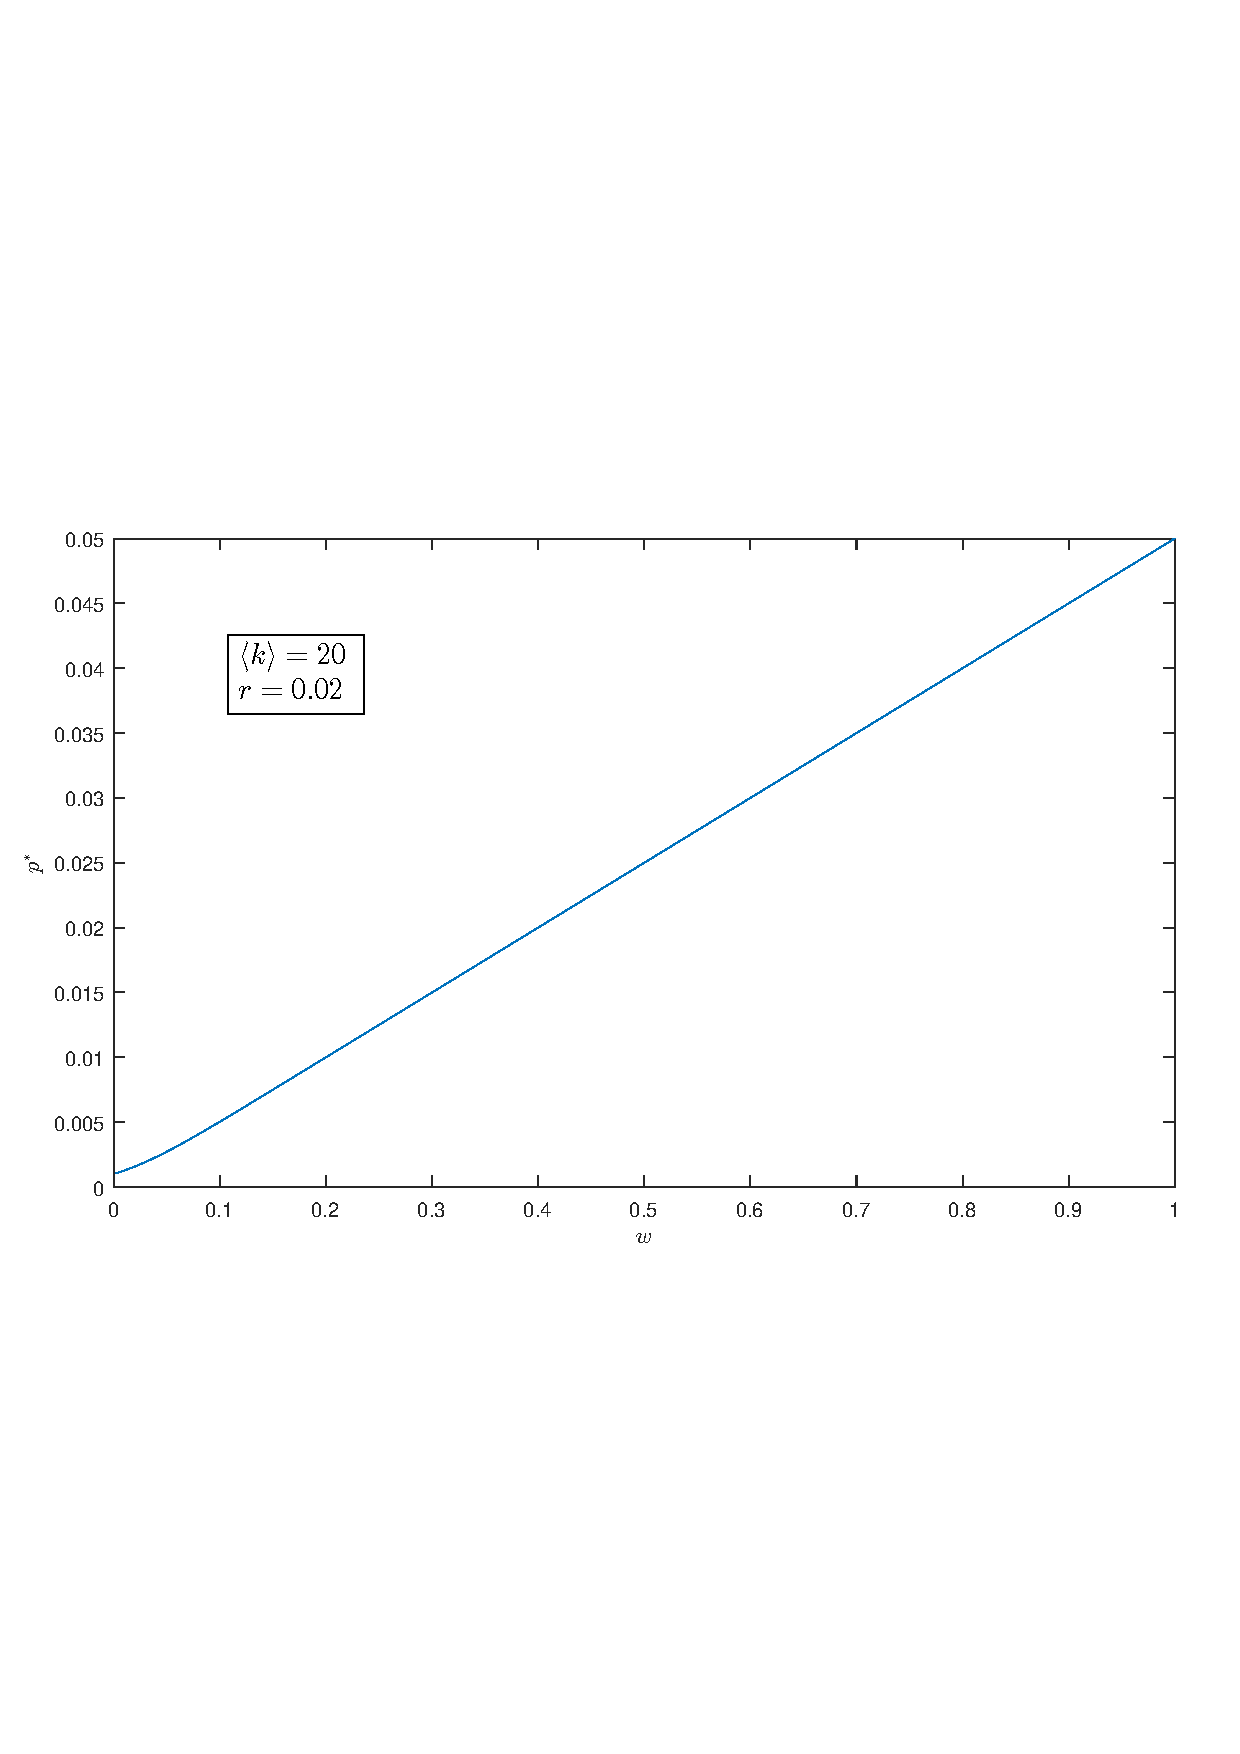
\includegraphics[bb=0bp 200bp 590bp 600bp,clip,scale=0.45]{soglia}
\par\end{center}

\end{frame}
%
\begin{frame}{Effetti del rewiring sulla topologia (1/2)}

\begin{textblock}{100}(10,15)Per indagare gli effetti del rewiring
sulla topologia consideriamo tre dinamiche distinte.
\begin{block}{}
\begin{itemize}
\item \textbf{1\textdegree{} caso}: rewiring casule.
\item \textbf{2\textdegree{} caso}: rewiring selettivo ma dinamica locale
assente.
\item \textbf{3\textdegree{} caso}: rewiring selettivo e dinamica locale
presente.
\end{itemize}
\end{block}
\end{textblock}
\begin{textblock}{42}(10,50)Il modello completo porta:
\begin{block}{}
\begin{itemize}
\item \textbf{Allargamento} della distribuzione di grado
\item \textbf{Assortatività}
\item \textbf{Separazione} tra suscettibli e infetti
\end{itemize}
\end{block}
\end{textblock}
\begin{textblock}{100}(57,50)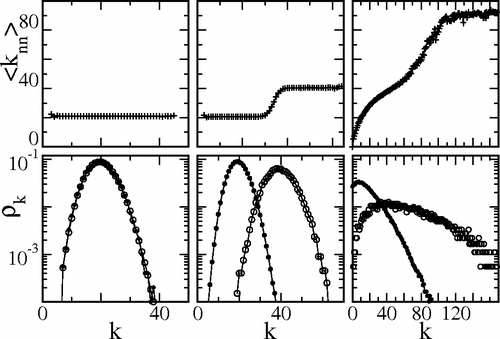
\includegraphics[scale=0.35]{medium}\end{textblock}

\end{frame}
%
\begin{frame}{Effetti del rewiring sulla topologia (2/2)}

\begin{textblock}{105}(10,15)

Un'analisi più raffinata può essere condotta considerando i \textbf{parametri
topologici} in funzione della probabilità di rewiring $w$.
\end{textblock}

\begin{textblock}{50}(8,30)

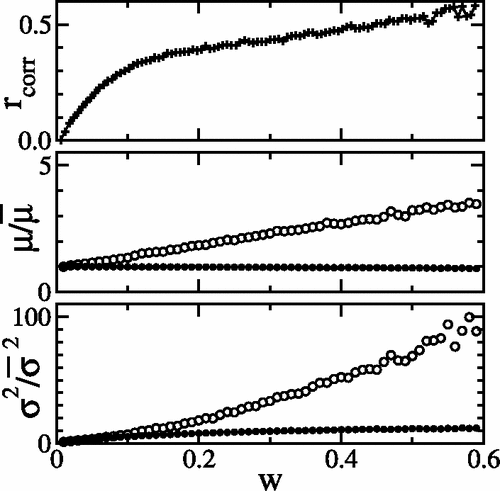
\includegraphics[scale=0.35]{medium2}
\end{textblock}

\begin{textblock}{50}(72,30)

All'aumentare di $w$:
\begin{block}{}
\begin{itemize}
\item Aumenta l'\textbf{assortatività.}
\item Aumenta la \textbf{media} della distribuzione di grado dei suscettibili
(cerchi).
\item Aumenta la \textbf{varianza} della distribuzione di grado dei suscettibili
(cerchi).
\end{itemize}
\end{block}
\end{textblock}

\end{frame}
%
\begin{frame}{Effetti globali del rewiring}

L'effetto del \textbf{rewiring} è duplice e contrapposto infatti:
\begin{itemize}
\item agisce sulla \textbf{dinamica locale} tendendo a far aumentare la
soglia epidemiologica.
\item crea una \textbf{dinamica topologica} tendendo a far aumentare la
varianza della distribuzione di grado perciò facendo diminuire la
soglia epidemiologica (che va come $\frac{r\left\langle k\right\rangle }{\left\langle k^{2}\right\rangle }$
in una \textbf{rete scale-free}).\pause
\end{itemize}
\medskip{}

Si instaura nella rete in questo modo una \textbf{dinamica complessa}
che è conveniente descrivere con un \textbf{modello di campo medio}.\pause
\begin{block}{Le variabili di stato di campo medio}
\begin{itemize}
\item $i$: densità degli infetti.
\item $l_{II}$: densità di link II.
\item $l_{SS}$: densità di link SS.
\end{itemize}
\end{block}
\end{frame}
%
\begin{frame}{Il modello di campo medio}

\begin{textblock}{60}(6,18)
\begin{block}{Il sistema di ODE}

\vspace{-0.3cm}

\[
\begin{cases}
\frac{\mathsf{d}i}{\mathsf{d}t}=pl_{SI}-ri\\
\frac{\mathsf{d}l_{II}}{\mathsf{d}t}=pl_{SI}\left(\frac{l_{SI}}{s}+1\right)-2rl_{II}\\
\frac{\mathsf{d}l_{SS}}{\mathsf{d}t}=(r+w)l_{SI}-\frac{2pl_{SI}l_{SS}}{s}
\end{cases}
\]
\end{block}
L'analisi di \textbf{biforcazione} rispetto a $p$ per i diversi valori
di $w$ mostra la presenza di \textbf{dinamiche complesse}:
\begin{block}{}
\begin{itemize}
\item \textbf{cicli di isteresi}
\item \textbf{bistabilità}
\item \textbf{dinamiche oscillatorie} (linee spesse).
\end{itemize}
\end{block}
\end{textblock}

\begin{textblock}{60}(71,18)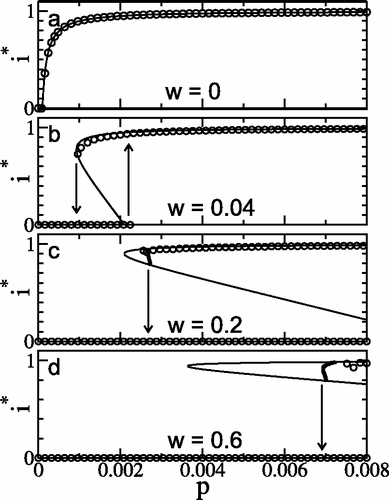
\includegraphics[scale=0.4]{medium3}\end{textblock}

\end{frame}
%
\begin{frame}{Analisi di biforcazione completa}

\vspace{-0.3cm}

\begin{center}
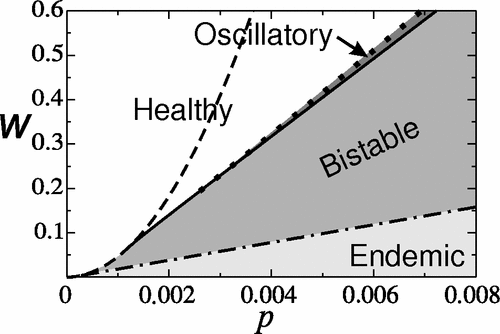
\includegraphics[scale=0.5]{medium4}
\par\end{center}

\vspace{-0.3cm}

\begin{block}{Legenda}

$-\cdot-\cdot-$ : \textbf{transcritica\qquad{}$----$ }:\textbf{
nodo sella}

\rule[0.5ex]{1.45cm}{1pt} : \textbf{Hopf\hspace{1.96cm}$\cdot\cdot\cdot\cdot\cdot\cdot\cdot\cdot$
}:\textbf{ tangente di cicli}
\end{block}
\end{frame}

\section{Conlusioni}
\begin{frame}[plain]
\begin{center}
\textbf{\LARGE{}Conclusioni}
\par\end{center}{\LARGE \par}

\end{frame}
%
\begin{frame}{Conclusioni}

\begin{textblock}{50}(10,10)
\begin{center}
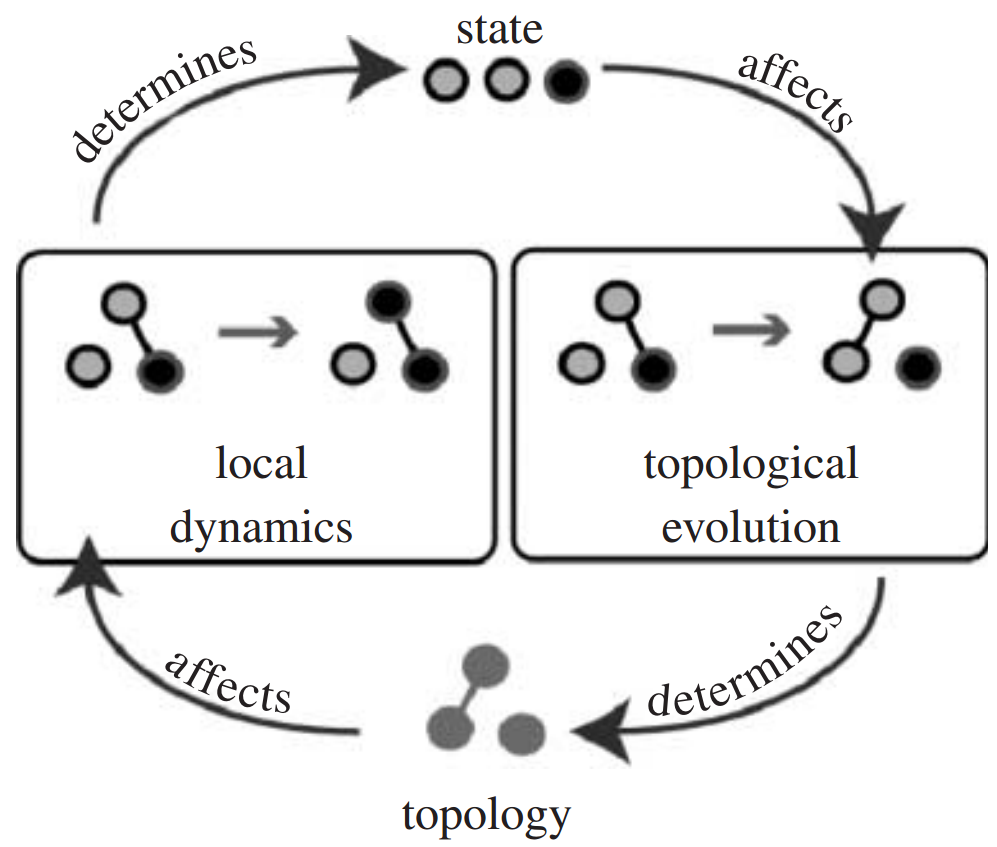
\includegraphics[scale=0.15]{feedback}
\par\end{center}

\vspace{-1cm}

\begin{center}
{\tiny{}Gross and Blasius, }\textit{\tiny{}J.R.Soc Interface}{\tiny{},
2007}
\par\end{center}{\tiny \par}

\end{textblock}

\begin{textblock}{55}(65,15)

Il modello presentato arricchisce la letteratura riguardante la dinamica
\textbf{su} e \textbf{di} reti complesse con un nuovo capitolo, mostrando
come l'\textbf{interazione} tra le due dinamiche porti alla formazione
di un \textbf{anello di retroazione} che produce dinamiche complesse.

\end{textblock}

\begin{textblock}{105}(10,65)

Ulteriori \textbf{raffinamenti} del modello sono possibili. Ad esempio:
\begin{itemize}
\item considerare la probabilità di rewiring $w$ come \textbf{funzione
della consapevolezza} della diffusione dell'epidemia e quindi della
densità di infetti $i$. {[}Gross e Kevrekidis, \textit{arXiv}, 2007{]}
\item \textbf{temporizzare} il rewiring. {[}Valdez \textit{et al}., \textit{Phys.
Rev. E}, 2012{]}
\end{itemize}
\end{textblock}
\end{frame}
%
\begin{frame}{Bibliografia}

{\footnotesize{}\bibliographystyle{plain}
\nocite{*}
\bibliography{EpidemicsAdaptiveNetwork}
}{\footnotesize \par}

\end{frame}

\appendix
%
\begin{frame}{Derivazione del modello di campo medio}

Derivata degli infetti: $\frac{\mathsf{d}i}{\mathsf{d}t}=pl_{SI}-ri$
\begin{itemize}
\item Aumento dovuto al contagio: $pl_{SI}$.
\item Diminuzione dovuta alla ripresa: $-ri$.
\end{itemize}
\begin{block}{Moment closure approximation}

$l_{ABC}=l_{AB}\mathsf{Pr}(BC|B)=l_{AB}\frac{l_{BC}}{B}$
\end{block}
Derivata dei link II: $\frac{\mathsf{d}l_{II}}{\mathsf{d}t}=pl_{SI}\left(\frac{l_{SI}}{s}+1\right)-2rl_{II}$
\begin{itemize}
\item Aumento dovuto al contagio da parte del nodo $i$: $pl_{SI}$.
\item Aumento dovuto al contagio di nodi $i$ collegati ad $s$: $\frac{pl_{SI}^{2}}{s}$.
\item Diminuzione dovuta alla ripresa dei nodi $i$: $-2rl_{II}$.
\end{itemize}
Derivata dei link SS: $\frac{\mathsf{d}l_{SS}}{\mathsf{d}t}=(r+w)l_{SI}-\frac{2pl_{SI}l_{SS}}{s}$
\begin{itemize}
\item Aumento dovuto alla ripresa degli infetti: $rl_{SI}$.
\item Aumento dovuto al rewiring: $wl_{SI}$.
\item Diminuzione dovuta al contagio $-\frac{2pl_{SI}l_{SS}}{s}$.
\end{itemize}
\end{frame}

\end{document}
